\documentclass[11pt]{article} 
\setlength{\oddsidemargin}{0.0in}
\setlength{\evensidemargin}{0.0in}
\setlength{\topmargin}{-0.25in}
\setlength{\headheight}{0in}
\setlength{\headsep}{0in}
\setlength{\textwidth}{6.5in}
\setlength{\textheight}{9.25in}
\setlength{\parindent}{0in}
\setlength{\parskip}{2mm}
\newcommand\tab[1][0.5cm]{\hspace*{#1}}
\usepackage{listings}
\usepackage{amsmath,amsfonts,amsthm, amssymb} % Math packages
\usepackage[utf8]{inputenc}
\usepackage{graphicx}
\usepackage{subcaption}
\usepackage{comment}

\title{ECS 189G Homework 2}
\author{Bochao Xin, Dianfeng Jiang, Melissa Goh, Shikun Huang}
\date{Due: 24 February 2020 (Monday)}

\begin{document}

\maketitle

\section{lm Model}
\subsection{Movienum}
Movienum will be our first predictor. But directly using movienum 
in lm function does not seem very promising, because movienum 
itself is only IDs for different movies and logically does not 
directly affect users' rating. Instead, we use movienum to 
calculate average rating of each individual movie. Then, we define 
movies with average ratings greater than or equal to 4.0 as 
"best movies" and define movies with average ratings less than or 
equal to 3.5 as "worst movies". Below is the code we used to do 
this job:
\begin{verbatim}
  # transform movienum to factor
  mov_factor <- as.factor(u.big$movienum) 
  levels <- levels(mov_factor)
  mov <- matrix(0,nrow = length(levels),ncol = 3)
  for (i in 1:length(levels)) {
    # find all the rows concerning the same movie
    movX <- u.big[mov_factor == levels[i],]
    average_rate <- mean(movX$rating)
    
    mov[i,1] <- as.numeric(levels[i])
    if(average_rate >= 4.0)
      mov[i,2] <- 1
    if(average_rate <= 3.5)
      mov[i,3] <- 1
  }
  mov <- as.data.frame(mov)
  names(mov) <- c("movienum","best_movie","worst_movie")
  
  # merge it back to data frame u.big later
  u.big <- merge(u.big, mov, by = "movienum", all.x = TRUE)
\end{verbatim}

Why did we do this? It comes from the intuition that some movies 
are just better than others. Those movies of high quality should 
receive higher scores than those of low quality. If most users 
speak highly of a certain movie, it proves that this movie is of 
high quality and tends to receive higher scores from future users, 
and vice versa.

\subsection{Usernum}
Our second predictor will be usernum. The way that we used to 
approach usernum is very similar to what we did for movienum. We 
use usernum to calculate average rating given by each individual 
user. Then, we define users who give average ratings less than or 
equal to 3.0 as "tough person" and define those who give average 
ratings greater than or equal to 4.0 as "nice person". Below is the 
code we used:
\begin{verbatim}
  usr_factor <- as.factor(u.big$usernum)
  levels <- levels(usr_factor)
  usr <- matrix(0,nrow=length(levels),ncol = 3)
  for (i in 1:length(levels)) {
    usrX <- u.big[usr_factor == levels[i],]
    average_rate <- mean(usrX$rating)
    usr[i,1] <- as.numeric(levels[i])
    
    if(average_rate >= 4.0)
      usr[i,2] <- 1
    if(average_rate <= 3.0)
      usr[i,3] <- 1
  }
  usr <- as.data.frame(usr)
  names(usr) <- c("usernum","nice_person","tough_person")
  u.big <- merge(u.big, usr, by = "usernum", all.x = TRUE)
\end{verbatim}

We did this because some users are just harsher than others, and 
they tend to give relative low ratings for movies they have seen.
Other users are just "nicer" than the ordinary, and they tend to
give relative high ratings for movies.

\subsection{Genres}
Different kinds of movies should affect their ratings. Our first 
attempt is to use all genres as predictors. Below is the result:
\begin{verbatim}
Call:
lm(formula = as.formula(indexToStr(u.big, predictors)), data = u.big.trn)

Residuals:
    Min      1Q  Median      3Q     Max 
-3.1872 -0.6248  0.2613  0.6814  2.1056 

Coefficients:
             Estimate Std. Error t value Pr(>|t|)    
(Intercept)  3.383414   0.011023 306.929  < 2e-16 ***
unknown     -0.272303   0.369749  -0.736 0.461457    
Action      -0.085943   0.010808  -7.952 1.86e-15 ***
Adventure    0.080097   0.012636   6.339 2.33e-10 ***
Animation    0.353127   0.024639  14.332  < 2e-16 ***
Children    -0.219328   0.018535 -11.833  < 2e-16 ***
Comedy      -0.064776   0.010340  -6.265 3.75e-10 ***
Crime        0.087370   0.013776   6.342 2.27e-10 ***
Documentary  0.250434   0.042608   5.878 4.18e-09 ***
Drama        0.241360   0.010050  24.017  < 2e-16 ***
Fantasy     -0.204901   0.033054  -6.199 5.71e-10 ***
FilmNoir     0.392378   0.029256  13.412  < 2e-16 ***
Horror      -0.132379   0.016954  -7.808 5.85e-15 ***
Musical      0.066690   0.018914   3.526 0.000422 ***
Mystery      0.114597   0.017160   6.678 2.43e-11 ***
Romance      0.113899   0.009462  12.037  < 2e-16 ***
SciFi        0.095209   0.012179   7.818 5.44e-15 ***
Thriller     0.019249   0.010444   1.843 0.065324 .  
War          0.258046   0.013124  19.663  < 2e-16 ***
Western      0.190491   0.027305   6.976 3.05e-12 ***
---
Signif. codes:  0 ‘***’ 0.001 ‘**’ 0.01 ‘*’ 0.05 ‘.’ 0.1 ‘ ’ 1

Residual standard error: 1.109 on 94980 degrees of freedom
Multiple R-squared:  0.03026,	Adjusted R-squared:  0.03007 
F-statistic:   156 on 19 and 94980 DF,  p-value: < 2.2e-16

[1] 0.8778 # MAPE
\end{verbatim}

\subsection{Occupations}
Our intuition to predicting ratings is based on factors that fundamentally represent the user's
personality. Some features we considered are age, usernum, and occupation. To elaborate on this,
we think that including usernum as a feature would let us know their rating based on how harshly
or leniently a user rates their movies, based on their user ID. 

\begin{figure}[ht!]
\begin{center}
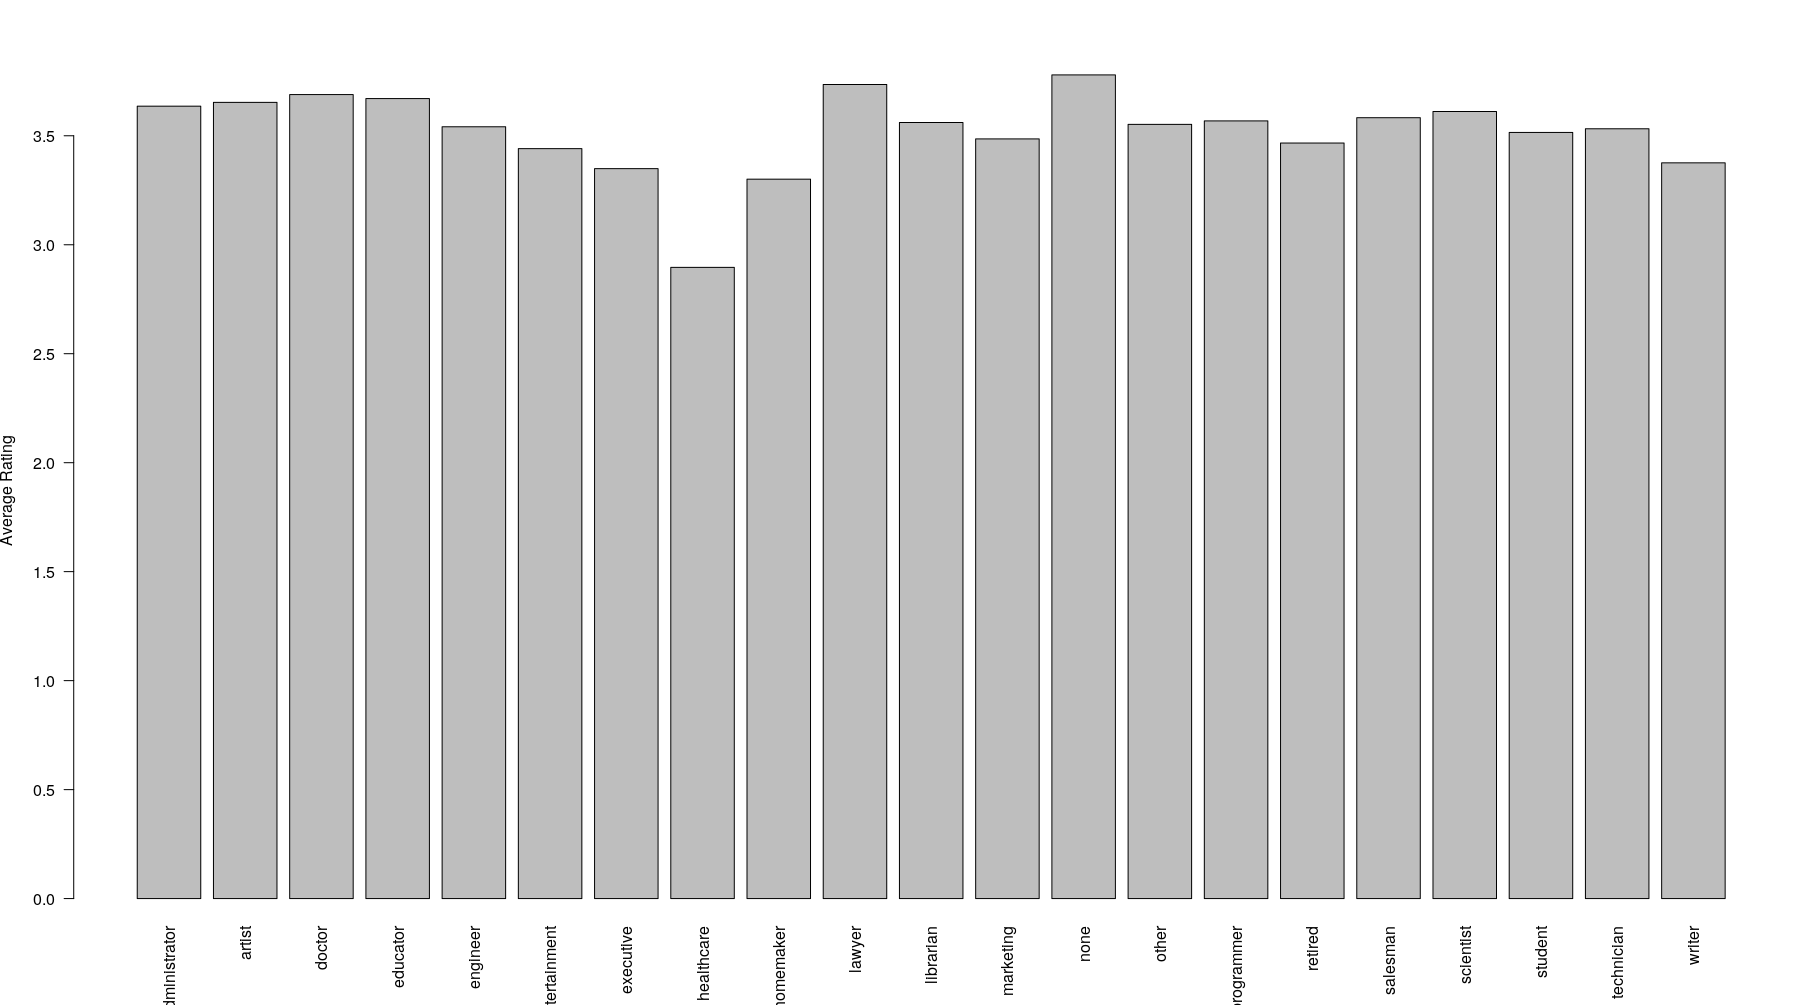
\includegraphics[width=0.8\textwidth]{ratingxocc.png}
\caption{Average Rating vs. Occupation}
\end{center}
\end{figure}

Intuitively, occupation reflects a person's personality. We plotted the average rating given by
each occupation. As shown in the plot, the ratings are not very uniform, which would probably
make Occupation a good feature to predict ratings. Since age likely affects
the kind of occupation a person has, we decided to use the interaction term `age` and `occ` to predicting
ratings. The MAPE obtained from this set of features is 0.8752.

\begin{verbatim}
    > lmout <- lm(rating ~ age*occ, data=trnSet)
    summary(lmout)
    > summary(lmout)
    
    Call:
    lm(formula = rating ~ age * occ, data = trnSet)
    
    Residuals:
        Min      1Q  Median      3Q     Max 
    -3.5559 -0.5763  0.3376  0.5374  2.8331 
    
    Coefficients:
                           Estimate Std. Error t value Pr(>|t|)    
    (Intercept)           3.3457294  0.0523707  63.885  < 2e-16 ***
    age                   0.0073463  0.0012955   5.670 1.43e-08 ***
    occartist            -0.6775732  0.1078113  -6.285 3.30e-10 ***
    occdoctor            -0.1125594  0.1831937  -0.614 0.538934    
    occeducator           0.3647334  0.0734661   4.965 6.89e-07 ***
    occengineer          -0.0359133  0.0688078  -0.522 0.601716    
    occentertainment      0.6526975  0.1318031   4.952 7.36e-07 ***
    occexecutive         -1.3817756  0.0913665 -15.123  < 2e-16 ***
    occhealthcare        -2.1325458  0.0901122 -23.665  < 2e-16 ***
    occhomemaker         -0.3012994  0.2346490  -1.284 0.199130    
    occlawyer             0.0806203  0.1262801   0.638 0.523199    
    occlibrarian          0.0534024  0.0785553   0.680 0.496629    
    occmarketing          0.3054019  0.1264570   2.415 0.015734 *  
    occnone               0.5380508  0.1263167   4.260 2.05e-05 ***
    occother              0.1970186  0.0646248   3.049 0.002299 ** 
    occprogrammer        -0.0590576  0.0695120  -0.850 0.395548    
    occretired           -0.3376369  0.4328787  -0.780 0.435404    
    occsalesman           0.1159735  0.1359053   0.853 0.393473    
    occscientist         -0.0424774  0.1416788  -0.300 0.764319    
    occstudent            0.2005008  0.0630880   3.178 0.001483 ** 
    occtechnician         0.2030625  0.0863610   2.351 0.018709 *  
    occwriter            -0.8011493  0.0768054 -10.431  < 2e-16 ***
    age:occartist         0.0247203  0.0032503   7.606 2.86e-14 ***
    age:occdoctor         0.0056768  0.0049181   1.154 0.248394    
    age:occeducator      -0.0083699  0.0017469  -4.791 1.66e-06 ***
    age:occengineer      -0.0007054  0.0017976  -0.392 0.694775    
    age:occentertainment -0.0267839  0.0043092  -6.216 5.14e-10 ***
    age:occexecutive      0.0302180  0.0023624  12.791  < 2e-16 ***
    age:occhealthcare     0.0360066  0.0022189  16.227  < 2e-16 ***
    age:occhomemaker      0.0009872  0.0068782   0.144 0.885874    
    age:occlawyer         0.0013949  0.0034506   0.404 0.686035    
    age:occlibrarian     -0.0031238  0.0019904  -1.569 0.116554    
    age:occmarketing     -0.0116446  0.0033326  -3.494 0.000476 ***
    age:occnone          -0.0114218  0.0045476  -2.512 0.012021 *  
    age:occother         -0.0071173  0.0017077  -4.168 3.08e-05 ***
    age:occprogrammer     0.0014500  0.0018701   0.775 0.438121    
    age:occretired        0.0001103  0.0070637   0.016 0.987546    
    age:occsalesman      -0.0038728  0.0037978  -1.020 0.307855    
    age:occscientist      0.0012039  0.0038758   0.311 0.756089    
    age:occstudent       -0.0085517  0.0020196  -4.234 2.29e-05 ***
    age:occtechnician    -0.0079412  0.0024493  -3.242 0.001186 ** 
    age:occwriter         0.0168032  0.0020383   8.244  < 2e-16 ***
    ---
    Signif. codes:  0 ‘***’ 0.001 ‘**’ 0.01 ‘*’ 0.05 ‘.’ 0.1 ‘ ’ 1
    
    Residual standard error: 1.109 on 94958 degrees of freedom
    Multiple R-squared:  0.02956,   Adjusted R-squared:  0.02914 
    F-statistic: 70.54 on 41 and 94958 DF,  p-value: < 2.2e-16
\end{verbatim}
\section{Problem B}

\end{document}